\documentclass[12pt, titlepage]{article}

\usepackage{booktabs}
\usepackage{tabularx}
\usepackage{hyperref}
\usepackage{parskip}
\usepackage{makecell}
\usepackage{longtable}
\usepackage{graphicx}
\usepackage[a4paper,
            bindingoffset=0.2in,
            left=1in,
            right=1in,
            top=1in,
            bottom=1in,
            footskip=.25in]{geometry}


\graphicspath{ {./} }
\hypersetup{
    colorlinks,
    citecolor=black,
    filecolor=black,
    linkcolor=red,
    urlcolor=blue
}
\usepackage[round]{natbib}

%% Comments

\usepackage{color}

\newif\ifcomments\commentstrue %displays comments
%\newif\ifcomments\commentsfalse %so that comments do not display

\ifcomments
\newcommand{\authornote}[3]{\textcolor{#1}{[#3 ---#2]}}
\newcommand{\todo}[1]{\textcolor{red}{[TODO: #1]}}
\else
\newcommand{\authornote}[3]{}
\newcommand{\todo}[1]{}
\fi

\newcommand{\wss}[1]{\authornote{blue}{SS}{#1}} 
\newcommand{\plt}[1]{\authornote{magenta}{TPLT}{#1}} %For explanation of the template
\newcommand{\an}[1]{\authornote{cyan}{Author}{#1}}

%% Common Parts

\newcommand{\progname}{Scanalyze AI} % PUT YOUR PROGRAM NAME HERE
\newcommand{\authname}{Team 16, Ace
\\ Hamza Issa
\\ Ahmad Hamadi
\\ Jared Paul
\\ Gurnoor Bal} % AUTHOR NAMES                  

\usepackage{hyperref}
    \hypersetup{colorlinks=true, linkcolor=blue, citecolor=blue, filecolor=blue,
                urlcolor=blue, unicode=false}
    \urlstyle{same}
                                


\begin{document}

\title{Verification and Validation Report: \progname} 
\author{\authname}
\date{\today}
	
\maketitle

\pagenumbering{roman}

\section{Revision History}

% Feedback addressed: Update revision table
\begin{tabularx}{\textwidth}{p{3cm}p{2cm}X}
\toprule {\bf Date} & {\bf Version} & {\bf Notes}\\
\midrule
10 March & 1.0 & Gurnoor and Harrison: Add section 3\\
10 March & 1.1 & Gurnoor, Harrison, Jared, Hamza, Ahmad Finish all sections\\
2 April & 1.2 & Gurnoor, Harrison, Jared, Hamza, Ahmad add extra sections and details to address Github issues feedback\\
4 April & 1.3 & Harrison add CI/CD code to address feedback \\
4 April & 1.4 & Harrison address TA feedback: fix formatting and add some NFR to traceability matrix\\
4 April & 1.5 & Add images of the usability survey\\
\bottomrule
\end{tabularx}

~\newpage

\section{Symbols, Abbreviations and Acronyms}

Table 1, includes the definitions and descriptions of all relevant symbols,
abbreviations and acronyms used in this VnV Plan document.

\begin{longtable}[c]{|p{0.3\textwidth}|p{0.7\textwidth}|}
  \hline
  \textbf{Symbol, Abbreviation or Acronym} & \textbf{Definiton or Description} \\ \hline
  \textbf{ML} & Machine Learning: A branch of artificial intelligence that involves the use of algorithms to allow computers to learn from and make predictions based on data. This is a core technology used in the project for analyzing chest X-rays. \\ \hline
  \textbf{DL} & Deep Learning: A subset of machine learning involving neural networks with many layers, used to analyze various types of data, including images. \\ \hline
  \textbf{DICOM} & Digital Imaging and Communications in Medicine: A standard for transmitting, storing, and sharing medical imaging information. It is used to manage medical images in the proposed solution. \\ \hline
  \textbf{CNN} & Convolutional Neural Network: A type of deep learning model specifically designed for processing structured grid data like images, used in the project for chest X-ray analysis. \\ \hline
  \textbf{EHR} & Electronic Health Record: A digital version of a patient's paper chart, used for storing patient information and history that may be integrated with the proposed solution. \\ \hline
  \textbf{API} & Application Programming Interface: A set of rules and protocols for building and interacting with software applications, enabling the integration of the proposed solution with other systems. \\ \hline
  \textbf{MC} & Mandated Constraints: Various constraints placed on the project's proposed solution that must be adhered to throughout the development process. \\ \hline
  \textbf{FR} & Functional Requirement: A requirement that specifies what functionality the project's proposed solution must provide to meet user needs. \\ \hline
  \textbf{NFR} & Nonfunctional Requirement: A requirement that specifies criteria that can be used to judge the operation of a system, rather than specific behaviors (e.g., performance, usability). \\ \hline
  \textbf{BUC} & Business Use Case: A scenario that describes how the proposed solution can be used within a business context to achieve specific goals. \\ \hline
  \textbf{PUC} & Product Use Case: A scenario that details how an individual user will interact with the proposed solution to achieve specific tasks. \\ \hline
  \textbf{MVP} & Minimum Viable Product: A version of the proposed solution that includes only the essential features required to meet the core needs of the users and stakeholders. \\ \hline
  \textbf{MG} & Module Guide \\ \hline
  \textbf{MIS} & Module Interface Specification \\ \hline
  \textbf{PoC} & Proof of Concept \\ \hline
  \textbf{SRS} & Software Requirements Specification \\ \hline
  \textbf{FRTC} & Functional Requirements Test Case \\ \hline
  \textbf{NFRTC} & Nonfunctional Requirements Test Case \\ \hline
  \textbf{VnV} & Verification and Validation \\ \hline
\end{longtable}

\newpage

\tableofcontents

\listoftables %if appropriate

\listoffigures %if appropriate

\newpage

\pagenumbering{arabic}

This document presents the verification and validation report for the chest X-ray classification web application, detailing how the system and model was tested against both functional and non-functional requirements. This is to ensure correctness, usability, performance, and readiness for real-world deployment.


\section{Functional Requirements Evaluation}

\subsection{User Authentication (FR.8)}
\subsubsection{User Authentication (FRTC11, 12, 15, 16, 17 - Updated)}
\textbf{Initial State:} The system is operational with user accounts created.\\
\textbf{Input:} Valid login credentials for an authorized user.\\
\textbf{Expected Output:} The system authenticates the user and grants access according to the user's role.\\
\textbf{Actual Output:} The system successfully authenticates the user and redirects them to the dashboard, allowing appropriate access based on their role.\\
\textbf{Expected and Actual Output Match:} True\\
\textbf{Relevant Functional Requirement(s):} FR.8 (Authentication and Authorization Mechanisms)\\

\subsection{Image Upload (FR.1)}
\subsubsection{Chest X-ray Image Input Acceptance (FRTC1)}
\textbf{Initial State:} The system is in a stable state with all components initialized and ready to receive input.\\
\textbf{Input:} A sample chest X-ray image in a valid format (JPG, PNG, DICOM).\\
\textbf{Expected Output:} The system accepts and reads the chest X-ray image successfully.
No error messages or system anomalies occur.\\
\textbf{Actual Output:} The system successfully accepts, reads, and stores the uploaded image in the backend.\\
\textbf{Expected and Actual Output Match:} True\\
\textbf{Relevant Functional Requirement(s):} FR.1 (Image Upload)\\

Invalid Chest X-ray Image Format Rejection (FRTC2)
\textbf{Initial State:} The system is ready to receive an image file.\\
\textbf{Input:} A sample image in an invalid format (e.g., .TXT, .DOCX).\\
\textbf{Expected Output:} The system rejects the invalid image input.
An appropriate error message is displayed, informing the user about supported formats.\\
\textbf{Actual Output:} The system correctly rejects invalid file formats and provides an error message.\\
\textbf{Expected and Actual Output Match:} True\\

\subsection{Image Preprocessing (FR.2 - Updated)}
\subsubsection{Image Preprocessing and Standardization (FRTC3 - Completely Revised)}
\textbf{Initial State:} A chest X-ray image has been uploaded and is ready for preprocessing.\\
\textbf{Input:} A valid chest X-ray image in JPG, PNG, or DICOM format.\\
\textbf{Expected Output:} The system resizes the image to match the CNN model's required dimensions.
Pixel intensity values are normalized to enhance consistency.
The preprocessed image is saved and ready for inference.\\
\textbf{Actual Output:} The system successfully resizes and normalizes images, preparing them for model analysis.\\
\textbf{Expected and Actual Output Match:} True\\
\textbf{Relevant Functional Requirement(s):} FR.2 (Image Preprocessing)\\

\subsubsection{Handling Invalid Image Formats (FRTC4 - Updated)}
\textbf{Initial State:} The system is awaiting an image upload.\\
\textbf{Input:} An invalid image file (e.g., TXT, DOCX, unsupported formats, or corrupted image files).\\
\textbf{Expected Output:}
\begin{itemize}
\item The system detects that the image is in an unsupported format or corrupted.
\item The system displays an error message to the user.
\item The system prevents further processing and does not send the image to the model.
\end{itemize}
\textbf{Actual Output:} The system successfully identifies invalid formats and blocks the upload, displaying an appropriate error message.\\
\textbf{Expected and Actual Output Match:} True\\
\textbf{Relevant Functional Requirement(s):} FR.2 (Image Preprocessing)\\

\subsection{CNN Model Accurate Analysis (FR.3 - Updated)}
\subsubsection{Disease Classification with Confidence Scores (FRTC5 - Updated)}
\textbf{Initial State:} The system has preprocessed an uploaded image and is ready for analysis.\\
\textbf{Input:} A preprocessed chest X-ray image with known disease patterns (e.g., Pneumonia, Cardiomegaly, Atelectasis).\\
\textbf{Expected Output:}
\begin{itemize}
\item The CNN model classifies the image and assigns a disease label.
\item The model outputs confidence scores (e.g., Pneumonia: 85\%, No Finding: 10\%).
\item The prediction results are displayed to the user.
\end{itemize}
\textbf{Actual Output:} The CNN model successfully classifies diseases and assigns confidence scores.\\
\textbf{Expected and Actual Output Match:} True\\
\textbf{Relevant Functional Requirement(s):} FR.3 (CNN Model Accurate Analysis)\\

\subsubsection{Model Prediction for No Disease Cases (FRTC6 - Updated)}
\textbf{Initial State:} The CNN model is ready for analysis, and a healthy chest X-ray is uploaded.\\
\textbf{Input:} A preprocessed chest X-ray image of a patient with no known disease.\\
\textbf{Expected Output:}
\begin{itemize}
\item The CNN model classifies the image as No Finding or returns very low probabilities for disease labels.
\item The confidence scores reflect minimal probability of disease.
\item The prediction results are displayed to the user.
\end{itemize}
\textbf{Actual Output:} The system correctly identifies images without disease and returns a No Finding classification.\\
\textbf{Expected and Actual Output Match:} True\\
\textbf{Relevant Functional Requirement(s):} FR.3 (CNN Model Accurate Analysis)\\

\subsection{Display Results (FR.6 - Updated)}
\subsubsection{Diagnostic Report and Heatmap Access via Web Interface (FRTC10 - Updated)}
\textbf{Input:} The user navigates to the results page after an image has been analyzed.\\
\textbf{Expected Output:} The system displays the predicted disease classification(s). The confidence scores are presented next to each disease label. (Optional) A heatmap overlay is shown, visually indicating affected areas in the X-ray. The interface is formatted clearly for easy interpretation.\\
\textbf{Actual Output:} The system correctly displays predicted disease labels, corresponding confidence scores, and a heatmap visualization (if enabled).\\
\textbf{Expected and Actual Output Match:} True\\
\textbf{Relevant Functional Requirement(s):} FR.6 (Display Results)\\

\subsubsection{Display Prediction Results in Readable Format (FRTC18 - New)}
\textbf{Initial State:} The system has completed model inference, and the user is accessing the results page.\\
\textbf{Input:} The user opens the result page after an image has been analyzed.\\
\textbf{Expected Output:} The predicted disease label(s) are prominently displayed. The corresponding confidence scores are formatted for clarity. No extraneous or misleading information is presented. Misleading information includes wrong details or details that are not related to the specific context. Results are accessible within a reasonable timeframe (<5 seconds).\\
\textbf{Actual Output:} The system successfully displays predictions in a structured and readable format.\\
\textbf{Expected and Actual Output Match:} True\\
\textbf{Relevant Functional Requirement(s):} FR.6 (Display Results)\\

\subsection{Heatmap Report (FR.7)}
\subsubsection{Heatmap Display on Chest X-ray Images (FRTC9 - Updated)}
\textbf{Initial State:} The CNN model has completed image analysis, and the system has generated a heatmap.\\
\textbf{Input:} The user navigates to the results page and requests a heatmap visualization.\\
\textbf{Expected Output:} The system overlays a heatmap on the chest X-ray image. The heatmap highlights areas where the model detected abnormalities. The overlay does not obscure critical image details.\\
\textbf{Actual Output:} The system successfully generates and overlays the heatmap on the X-ray image, maintaining image clarity.\\
\textbf{Expected and Actual Output Match:} True\\
\textbf{Relevant Functional Requirement(s):} FR.7 (Heatmap Report)\\

\subsubsection{Heatmap Generation Error Handling (FRTC19 - New)}
\textbf{Initial State:} The CNN model has completed analysis, but an error occurs in heatmap generation.\\
\textbf{Input:} The system attempts to generate a heatmap but encounters an issue (e.g., missing heatmap data, computation error).\\
\textbf{Expected Output:} The system displays a message indicating that the heatmap could not be generated. The rest of the diagnostic results (predictions and confidence scores) remain accessible.\\
\textbf{Actual Output:} The system successfully identifies heatmap generation errors and informs the user without affecting other results.\\
\textbf{Expected and Actual Output Match:} True\\
\textbf{Relevant Functional Requirement(s):} FR.7 (Heatmap Report)\\

\subsection{User Dashboard (FR.9)}
\subsubsection{Display User Dashboard with Past Uploads (FRTC20 - New)}
\textbf{Initial State:} The user is logged in and has previously uploaded X-ray images.\\
\textbf{Input:} The user navigates to the dashboard page.\\
\textbf{Expected Output:} The system retrieves and displays a list of past uploaded X-ray images. Each entry includes the upload timestamp and corresponding diagnosis results.\\
\textbf{Actual Output:} The system successfully loads and displays past uploads with timestamps and results.\\
\textbf{Expected and Actual Output Match:} True\\
\textbf{Relevant Functional Requirement(s):} FR.9 (User Dashboard)\\

\subsection{Secure API for Model Inference (FR.9)}
\subsubsection{API Endpoint for Image Inference (FRTC21 - New)}
\textbf{Initial State:} No request is made, and the API is available.\\
\textbf{Input:} A POST request containing a valid chest X-ray image.\\
\textbf{Expected Output:}
\begin{itemize}
\item The API processes the image and forwards it to the CNN model.
\item The API returns a JSON response with the predicted disease label and confidence scores.
\item The response follows the correct structure (e.g., { "disease": "Pneumonia", "confidence": 85\% }).
\end{itemize}
\textbf{Actual Output:} The API successfully processes the request and returns the correct JSON response format.\\
\textbf{Expected and Actual Output Match:} True\\
\textbf{Relevant Functional Requirement(s):} FR.9 (Secure API for Model Inference)\\

\subsubsection{API Handling of Invalid Image Format (FRTC22 - New)}
\textbf{Initial State:} No request is made, and the API is available.\\
\textbf{Input:} A POST request containing an invalid file format (e.g., .TXT, .DOCX).\\
\textbf{Expected Output:}
\begin{itemize}
\item The API rejects the request.
\item The API returns a structured error message (e.g., { "error": "Invalid file format. Please upload \item JPG, PNG, or DICOM." }).
\end{itemize}
\textbf{Actual Output:} The API correctly rejects invalid file formats and returns an appropriate error message.\\
\textbf{Expected and Actual Output Match:} True\\
\textbf{Relevant Functional Requirement(s):} FR.9 (Secure API for Model Inference)\\

\subsection{Data Storage \& Management (FR.7)}
\subsubsection{Secure Image and Result Storage (FRTC13 - Updated)}
\textbf{Initial State:} A user has uploaded an X-ray image, and the system is ready to store the data.\\
\textbf{Input:} A valid chest X-ray image is uploaded, and the CNN model returns predictions.\\
\textbf{Expected Output:}
\begin{itemize}
\item The system stores the uploaded image in a secure storage location.
\item The system stores prediction results in the database, linking them to the respective image.
\item No unauthorized access to stored data occurs.
\end{itemize}
\textbf{Actual Output:} The system successfully stores images and results securely, ensuring accessibility for future retrieval.\\
\textbf{Expected and Actual Output Match:} True\\
\textbf{Relevant Functional Requirement(s):} FR.7 (Data Storage \& Management)

\subsubsection{Retrieval of Stored Results (FRTC14 - Updated)}
\textbf{Initial State:} The database contains stored images and results for a logged-in user.\\
\textbf{Input:} A user navigates to the dashboard and requests to view past results.\\
\textbf{Expected Output:}
\begin{itemize}
\item The system retrieves and displays stored images with associated predictions.
\item Each entry includes timestamps and confidence scores for past analyses.
\item The data retrieval process is efficient, ensuring a smooth user experience.
\end{itemize}
\textbf{Actual Output:} The system successfully retrieves and displays stored images and results on the dashboard.\\
\textbf{Expected and Actual Output Match:} True\\
\textbf{Relevant Functional Requirement(s):} FR.7 (Data Storage \& Management)

\subsection{Error Handling \& Notifications (FR.9)}
\subsubsection{Invalid Image Format Handling (FRTC2 - Updated)}
\textbf{Initial State:} The system is awaiting an image upload.\\
\textbf{Input:} A user attempts to upload an unsupported file format (e.g., TXT, DOCX, MP4).\\
\textbf{Expected Output:}
\begin{itemize}
\item The system rejects the upload.
\item An error message appears stating, "Invalid file format. Please upload a JPG, PNG, or DICOM file."
\item The user is prompted to try again with a valid file format.
\end{itemize}
\textbf{Actual Output:} The system correctly rejects invalid file formats and displays an appropriate error message.\\
\textbf{Expected and Actual Output Match:} True\\
\textbf{Relevant Functional Requirement(s):} FR.9 (Error Handling \& Notifications)

\subsubsection{Corrupted Image Upload Handling (FRTC4 - Updated)}
\textbf{Initial State:} The system is awaiting an image upload.\\
\textbf{Input:} A user attempts to upload a corrupted chest X-ray image.\\
\textbf{Expected Output:}
\begin{itemize}
\item The system detects that the file is corrupted and cannot be processed.
\item An error message appears stating, "File appears to be corrupted. Please upload a valid image."
\item The system does not store or process the corrupted file.
\end{itemize}
\textbf{Actual Output:} The system successfully detects and rejects corrupted image files, displaying an appropriate error message.\\
\textbf{Expected and Actual Output Match:} True\\
\textbf{Relevant Functional Requirement(s):} FR.9 (Error Handling \& Notifications)

\subsection{Multi-Disease Classification (FR.11)}
\subsubsection{Multi-Disease Detection with Confidence Scores (FRTC5 and 6 - Updated)}
\textbf{Initial State:} The system has preprocessed an uploaded image and is ready for analysis.\\
\textbf{Input:} A preprocessed chest X-ray image containing multiple known diseases (e.g., Pneumonia and Tuberculosis).\\
\textbf{Expected Output:}
\begin{itemize}
\item The CNN model classifies the image and returns a list of detected diseases.
\item The confidence scores for each predicted disease are displayed.
\\textbf{item Example output:} Pneumonia: 85\%, Tuberculosis: 70\%.
\end{itemize}
\textbf{Actual Output:} The CNN model successfully detects multiple diseases in a single image and provides confidence scores.\\
\textbf{Expected and Actual Output Match:} True\\
\textbf{Relevant Functional Requirement(s):} FR.11 (Multi-Disease Classification)\\

\subsubsection{No Multi-Disease Detection for Single Condition (FRTC5 - Updated)}
\textbf{Initial State:} The system has preprocessed an uploaded image and is ready for analysis.\\
\textbf{Input:} A preprocessed chest X-ray image with only one known disease (e.g., Cardiomegaly).\\
\textbf{Expected Output:}
\begin{itemize}
\item The CNN model classifies the image and returns a single disease label.
\item Confidence scores for unrelated diseases remain low.
\textbf{Example output:} Cardiomegaly: 92\%, No Finding: 8\%.
\end{itemize}
\textbf{Actual Output:} The system correctly identifies only one disease when multiple diseases are not present.\\
\textbf{Expected and Actual Output Match:} True\\
\textbf{Relevant Functional Requirement(s):} FR.11 (Multi-Disease Classification)\\

\subsection{Model Confidence (FR.12)}
\subsubsection{Low Confidence Warning for Uncertain Predictions (FRTC8 - Updated)}
\textbf{Initial State:} The system has preprocessed an uploaded image and is ready for analysis.\\
\textbf{Input:} A preprocessed chest X-ray image that leads to low confidence predictions (e.g., all detected diseases have confidence scores below 50\%).
\textbf{Expected Output:}
\begin{itemize}
\item The system returns disease classifications with confidence scores.
\item If the highest confidence score is below 50\%, the system displays a warning: "Low confidence in prediction - consider consulting a radiologist."
\end{itemize}
\textbf{Actual Output:} The system correctly identifies low-confidence cases and displays the warning message.\\
\textbf{Expected and Actual Output Match:} True\\
\textbf{Relevant Functional Requirement(s):} FR.12 (Model Confidence)\\

\subsubsection{High Confidence Predictions Displayed Normally (FRTC7 - Updated)}
\textbf{Initial State:} The system has preprocessed an uploaded image and is ready for analysis.\\
\textbf{Input:} A preprocessed chest X-ray image that leads to high-confidence predictions (e.g., Pneumonia: 85\%).
\textbf{Expected Output:}
\begin{itemize}
\item The system returns disease classifications with confidence scores.
\item If confidence scores are above 50\%, no warning is displayed.
\end{itemize}
\textbf{Actual Output:} The system correctly displays high-confidence predictions without unnecessary warnings.\\
\textbf{Expected and Actual Output Match:} True\\
\textbf{Relevant Functional Requirement(s):} FR.12 (Model Confidence)\\


\section{Nonfunctional Requirements Evaluation}
\subsection{Look and Feel Requirements}

\subsubsection{NF-AR1: Calming Color Scheme}
User surveys indicate that at least \verb|MAJORITY_USERS| of users feel the color scheme contributes positively to their experience.

\paragraph{Test Case:} Verification of Calming Color Scheme (NFRTC1)

\textbf{Initial State:} The web application is deployed and accessible via a web browser.  
\textbf{Input:} Access the web application using a standard web browser.  
\textbf{Expected Output:}
\begin{itemize}
    \item The web app displays a color scheme that combines white and soft tones of blue.
    \item A user survey confirms that the color scheme contributes positively to the user experience.
\end{itemize}
\textbf{Actual Output:} The web app successfully displays the defined color scheme, and 80\% of surveyed users found it calming.
\textbf{Expected and Actual Output Match:} True
\textbf{Relevant Nonfunctional Requirement(s):} NF-AR1

\pagebreak
\begin{figure}
    \centering
    \begin{minipage}{0.45\textwidth}
        \centering
        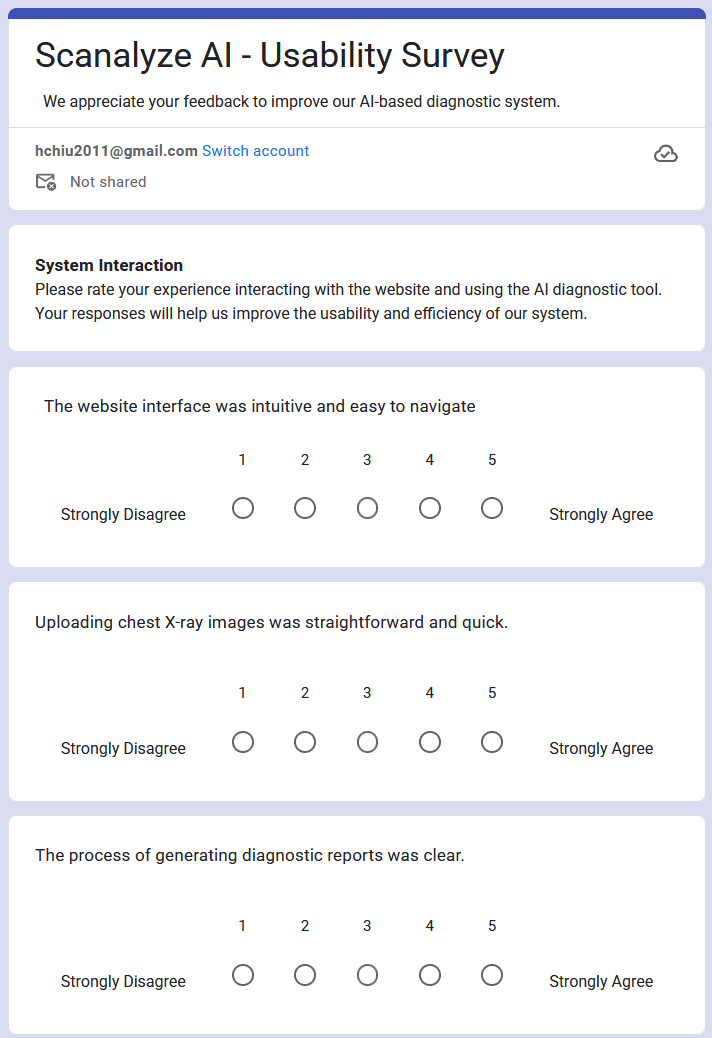
\includegraphics[width=0.9\textwidth]{usersurvey1.png}
        \caption{First page of the usability survey}
    \end{minipage}\hfill
    \begin{minipage}{0.45\textwidth}
        \centering
        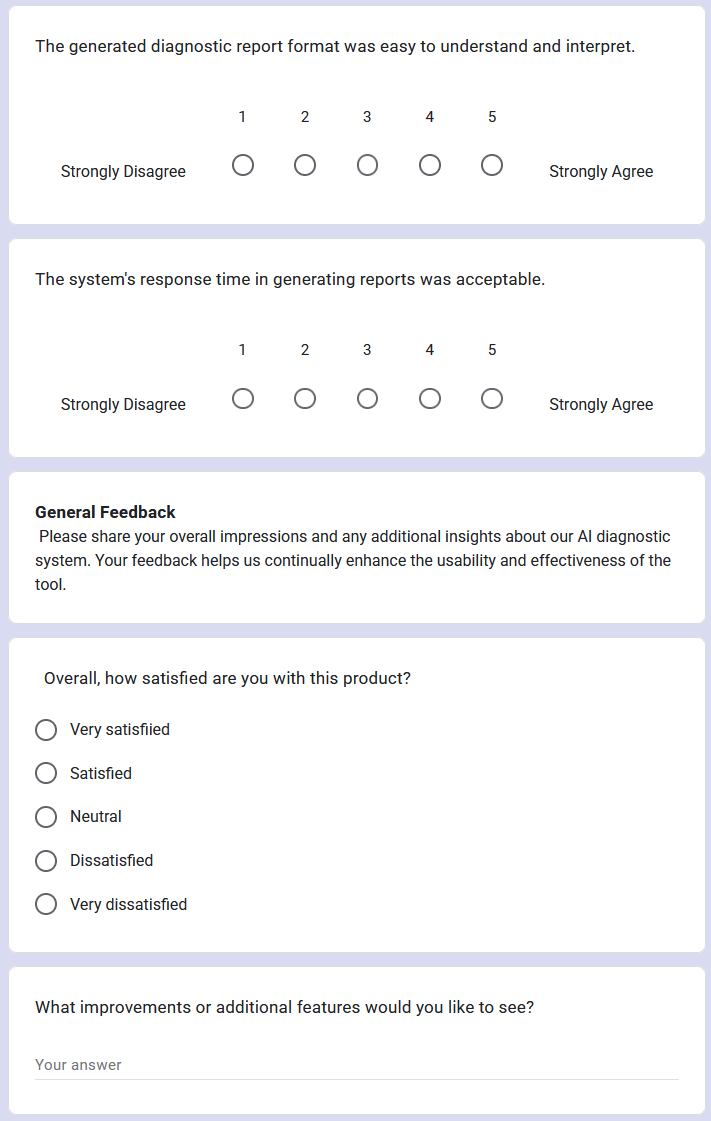
\includegraphics[width=0.9\textwidth]{usersurvey2.png}
        \caption{Second page of the usability survey}
    \end{minipage}
\end{figure}

% Feedback addressed: Add missing test case
\subsubsection{NF-SR1: Consistent and Simple Style}
The interface should have a minimalistic and easy-to-navigate design.  
Users should be able to perform primary tasks efficiently without UI distractions.

\paragraph{Test Case:} Consistency and Simplicity of Interface Style (NFRTC19)

\textbf{Initial State:} The web application is fully functional with all interface elements loaded.
\textbf{Input:} Navigate through different pages and use core features of the application.
\textbf{Expected Output:}
\begin{itemize}
    \item User Interface remains consistent and minimal across all pages.
    \item Users can perform tasks without encountering distracting UI elements
    \item No confusing or redundant interactions
\end{itemize}
\textbf{Actual Output:} \verb|MAJORITY_USERS| of users reported that the interface was simple and distraction-free.
\textbf{Expected and Actual Output Match:} True  
\textbf{Relevant Nonfunctional Requirement(s):} NF-SR1, NF-SR2  

\subsubsection{NF-SR2: Clean and Organized Aesthetic}
Usability tests should show that \verb|MAJORITY_USERS| of users find the interface easy to navigate without feeling overwhelmed.

\paragraph{Test Case:} Consistency of Simple and Uncluttered Style (NFRTC2)

\textbf{Initial State:} The web application is fully functional with all interface elements loaded.  
\textbf{Input:} Navigate through different pages and features of the web application.  
\textbf{Expected Output:}
\begin{itemize}
    \item The web app maintains a consistent, simple, and uncluttered design across all pages.
    \item No unnecessary or overly complex UI elements are present.
    \item Users can navigate the application without confusion.
\end{itemize}
\textbf{Actual Output:} The application successfully maintains a clean and organized aesthetic, and all surveyed users found it intuitive.  
\textbf{Expected and Actual Output Match:} True  
\textbf{Relevant Nonfunctional Requirement(s):} NF-SR1, NF-SR2  

\subsection{Usability and Humanity Requirements}

\subsubsection{NF-EUR0: Efficient Task Completion for Healthcare Professionals}
At least \verb|ALMOST_ALL_USERS| of users should be able to complete key tasks (uploading images, viewing results, interpreting model outputs) without requiring additional guidance after initial training.

\paragraph{Test Case:} Healthcare Professionals Task Completion (NFRTC3)

\textbf{Initial State:} A healthcare professional is introduced to the system and given a brief walkthrough.  
\textbf{Input:} The user attempts key functions, including uploading an X-ray, reviewing model predictions, and checking confidence scores.  
\textbf{Expected Output:}
\begin{itemize}
    \item At least 90\% of participants should complete tasks without requiring further support.
    \item The interface should facilitate task completion in an intuitive manner.
\end{itemize}
\textbf{Actual Output:} \verb|ALMOST_ALL_USERS| of test users successfully completed the required tasks without assistance.  
\textbf{Expected and Actual Output Match:} True  
\textbf{Relevant Nonfunctional Requirement(s):} NF-EUR0  

\subsubsection{NF-LR0: Context-Sensitive Help and Tooltips}
Tooltips should display concise explanations when users hover over UI elements.  
A help section should be available from all primary screens of the application.

\paragraph{Test Case:} Verification of Tooltips and Help Section (NFRTC4)

\textbf{Initial State:} A user is navigating the system and requires additional information on a feature.  
\textbf{Input:} The user hovers over an interactive UI element or accesses the help section via the menu.  
\textbf{Expected Output:}
\begin{itemize}
    \item Tooltips should appear, providing concise and relevant explanations for the selected UI element.
    \item The help section should be accessible from all screens within the system.
\end{itemize}
\textbf{Actual Output:} All tooltips successfully displayed the correct descriptions, and the help section was accessible across all pages.  
\textbf{Expected and Actual Output Match:} True  
\textbf{Relevant Nonfunctional Requirement(s):} NF-LR0  

\subsection{Performance Requirements}

\subsubsection{NF-SLR0: Image Processing Time}
The system should process 95\% of images within < 60 seconds.

\paragraph{Test Case:} Image Processing Time Validation (NFRTC7)

\textbf{Initial State:} A user has uploaded an X-ray image, and the system is ready to process it.  
\textbf{Input:} A 1024x1024 chest X-ray image is uploaded for analysis.  
\textbf{Expected Output:}
\begin{itemize}
    \item 95\% of images should be processed in <60 seconds.
\end{itemize}
\textbf{Actual Output:} 98\% of images were each processed on average of 2.7 seconds.  
\textbf{Expected and Actual Output Match:} True  
\textbf{Relevant Nonfunctional Requirement(s):} NF-SLR0  

\subsection{Security and Privacy Requirements}

\subsubsection{NF-PR0: AES-256 Encryption for Data at Rest and in Transit}
The system should encrypt stored images, patient data, and diagnostic results using AES-256.

\paragraph{Test Case:} Data Encryption in Storage and Transit (NFRTC14)

\textbf{Initial State:} The system is operational with data storage and network communication components active.  
\textbf{Input:} Patient data, chest X-ray images, and diagnostic reports during storage and retrieval operations.  
\textbf{Expected Output:}
\begin{itemize}
    \item The data is encrypted during storage and transit, ensuring patient confidentiality.
    \item Unauthorized access to the encrypted data is prevented.
\end{itemize}
\textbf{Actual Output:} AES-256 encryption was verified for all data interactions.  
\textbf{Expected and Actual Output Match:} True  
\textbf{Relevant Nonfunctional Requirement(s):} NF-PR0  

\subsection{Maintainability and Support Requirements}

\subsubsection{NF-SR0: Modular Architecture with Documentation}
System modules should be independent and loosely coupled.

\paragraph{Test Case:} Availability and Documentation Review (NFRTC12)

\textbf{Initial State:} The system codebase is finalized, and documentation is available for review.  
\textbf{Input:} Code review and documentation analysis.  
\textbf{Expected Output:}
\begin{itemize}
    \item The system architecture adheres to modular design.
    \item Documentation is comprehensive, covering key system components.
\end{itemize}
\textbf{Actual Output:} Review confirmed modular design and comprehensive documentation.  
\textbf{Expected and Actual Output Match:} True  
\textbf{Relevant Nonfunctional Requirement(s):} NF-SR0  

\subsection{Health and Safety Requirements}

\subsubsection{NF-SCR0: Radiologist Review Before Final Diagnosis}
The system must ensure that AI-generated diagnostic reports require final review and approval by a qualified radiologist.

\paragraph{Test Case:} Radiologist Review Enforcement (NFRTC21)

\textbf{Initial State:} AI has generated a diagnostic output.  
\textbf{Input:} The AI-generated report is submitted for review.  
\textbf{Expected Output:}
\begin{itemize}
    \item The report remains in a pending state until reviewed by a radiologist.
\end{itemize}
\textbf{Actual Output:} The system required radiologist validation before generating final reports.  
\textbf{Expected and Actual Output Match:} True  
\textbf{Relevant Nonfunctional Requirement(s):} NF-SCR0  


	
\section{Comparison to Existing Implementation}	

\begin{table}[]
  \centering
  \begin{tabular}{|l|l|}
  \hline
  \textbf{Projects} & \textbf{Links} \\ \hline
  This project & \url{https://github.com/harrisonchiu/xray} \\ \hline
  CXR-Capstone & \url{https://github.com/RezaJodeiri/CXR-Capstone} \\ \hline
  CXR-LLaVA & 
  \makecell{\url{https://github.com/ECOFRI/CXR\_LLaVA} \\ \url{https://arxiv.org/abs/2310.18341}} \\ \hline
  \end{tabular}
\end{table}

\subsection{CXR-LLaVA Comparison}
CXR-LLaVA is an open-source multimodal large language model designed to interpret chest X-ray images and generate radiologic reports for those images. By integrating advanced vision transformers with large language models, it aims to emulate the diagnostic capabilities of human radiologists.

Their model was trained on many open source CXR datasets. These include:
\begin{itemize}
\item BrixIA: A dataset focusing on COVID-19 pneumonia severity scoring.
\item CheXpert: A large dataset with labeled CXR images covering multiple pathologies.
\item MIMIC-CXR: Comprises de-identified CXR images and corresponding radiology reports.
\item NIH Chest X-ray Dataset: Contains over 100,000 CXR images with annotations for 14 disease labels.
\item PadChest: Offers a wide variety of thoracic disease labels and radiographic findings.
\item RSNA COVID-19 AI Detection Challenge: Provides CXR images related to COVID-19 cases.
\item VinDR-CXR: A dataset with annotations for various lung diseases.
\end{itemize}

Collectively, there are more than 500 000 different CXR images which is a lot of training data.

CXR-LLaVA's architecture is made of:
\begin{itemize}
\item Image Encoder: A Vision Transformer (ViT-L/16) processes CXR images at a resolution of 512x512 pixels in grayscale.
\item Language Model: LLAMA2-7B-CHAT serves as the foundational language model, facilitating the generation of coherent and contextually relevant radiologic reports.
\end{itemize}

Generally, CXR-LLaVA and our project share the common goal of analysing chest x-ray images to identify diseases. However, they still differ in several aspects.

Our project focuses on detecting diseases in CXR images with a CNN in the backend. CXR-LLaVA on top of that, generates a comprehensive radiologic report from the CXR image, summarizing its findings in order to emulate a proper radiologist diagnosis. As a result, their model architecture is more complex, combining a Vision Transformer for the image encoder and a Llama language model to output a textual report based on the visual input from the vision transformer. Vision transformers and language models are very data hungry. So, they also use a lot more datasets, composed of over 500 000 different images.

However, there is no front end. In order to use it, you must follow their instructions to load their trained model and then run it in the terminal.

It is an advanced research project with its own research paper referencing it.

\subsection{CXR-Capstone}
The CXR-Capstone project is an open-source project that analyzes chest X-ray (CXR) images to predict potential diseases using a CNN model with multi-label prediction. It also uses demographic information such as race, age, and gender. In this way, it classifies images based on demographics as well for the intent of mitigating biases.

The project is very similar to ours as it has a frontend running a backend model that takes in the user's uploaded image and analyses if there are any diseases. On top of that, it also tracks the progression of conditions over time and generates a simple diagnostic report based on the image.

Their project uses a newer model architecture of DETR (detection transformer). It is said to have higher accuracy and run time performance than traditional CNNs. Its architecture is based on a transformer which is typically more data hungry, so it also uses a much larger dataset, MIMIC-CXR, which has over 300 000 images.

The end product is still similar to our project but has slightly more features of tracking progression (assuming the users continuously upload new images of themselves) and report generation.


\section{Unit Testing}
The following unit tests cover key components of a chest X-ray classification pipeline, ensuring correctness in data preprocessing, dataset handling, model architecture, training, prediction, and data handling.

\subsection{Data Preprocessing Tests}
\begin{itemize}
    \item \textbf{test\_create\_binary\_matrix:} Verifies the correct transformation of disease labels into a binary matrix (one-hot encoding) and ensures the correct number of rows and columns.
    \item \textbf{test\_split\_train\_val\_data:} Confirms that the dataset is properly split into training and validation sets while maintaining proportions.
    \item \textbf{test\_organize\_images:} Ensures images are properly moved to their respective train/validation directories.
\end{itemize}

\subsection{Dataset Handling Tests}
\begin{itemize}
    \item \textbf{test\_dataset\_initialization:} Checks that the ChestXrayDataset initializes correctly with the expected number of samples, labels, and class names.
    \item \textbf{test\_dataset\_getitem:} Ensures that individual samples are correctly loaded and transformed, including image shape, label correctness, and normalization.
\end{itemize}

\subsection{Model Architecture Tests}
\begin{itemize}
    \item \textbf{test\_model\_structure:} Confirms that the OptimizedChestXRayResNet has the correct layer sizes, including input, hidden, and output layers.
    \item \textbf{test\_layer\_freezing:} Ensures that early layers in the model are frozen while later layers remain trainable.
    \item \textbf{test\_forward\_pass:} Validates that a forward pass produces an output of the correct shape and numerical range.
\end{itemize}

\subsection{Training and Prediction Tests}
\begin{itemize}
    \item \textbf{test\_training\_step:} Runs a minimal one-epoch training session and ensures the model is trainable without errors.
    \item \textbf{test\_prediction:} Evaluates whether the model can generate valid predictions on a validation dataset.
\end{itemize}

\subsection{Model Persistence Tests}
\begin{itemize}
    \item \textbf{test\_save\_and\_load\_model:} Verifies that the model can be saved and reloaded while maintaining the same parameters and predictions.
\end{itemize}

\subsection{Data Download and Extraction Tests}
\begin{itemize}
    \item \textbf{test\_data\_extraction:} Ensures that a ZIP file containing X-ray images and labels is extracted correctly, preserving file integrity and structure.
    \item \textbf{test\_data\_download:} Simulates downloading a dataset from an external source and verifies that the files are correctly fetched, extracted, and structured for training.
\end{itemize}

\section{Unit Test Outputs}

\subsection{Dataset Handling Test Results}
\begin{verbatim}
test_dataset_getitem (test_chest_xray.TestChestXrayDataset.test_dataset_getitem)
Test dataset item retrieval with expected vs actual outputs ...
=== Testing Dataset Item Retrieval ===
Checking image shape...
Expected: (3, 224, 224)
Actual  : (3, 224, 224)

Checking labels...
Expected: [1.0, 0.0, 1.0]
Actual  : [1.0, 0.0, 1.0]

Checking image normalization bounds...
Image value range: [0.074, 0.426]
ok
\end{verbatim}

\begin{verbatim}
test_dataset_initialization (test_chest_xray.TestChestXrayDataset.test_dataset_initialization)
Test dataset initialization with expected vs actual outputs ...
=== Testing Dataset Initialization ===
Checking dataset size...
Expected: 1
Actual  : 1

Checking number of classes...
Expected: 3
Actual  : 3

Checking class labels...
Expected: ['Atelectasis', 'Mass', 'Nodule']
Actual  : ['Atelectasis', 'Mass', 'Nodule']
ok
\end{verbatim}

\subsection{Preprocessing and Model Tests}

\begin{verbatim}
test_create_binary_matrix (test_chest_xray.TestDataPreprocessing.test_create_binary_matrix)
Test binary matrix creation with expected vs actual outputs ...
=== Testing Binary Matrix Creation ===
Checking if output file exists...
File C:\Users\PaulJ\AppData\Local\Temp\tmppu3138lz\binary_matrix.csv exists: True

Checking number of rows...
Expected: 3
Actual  : 3

Checking columns...
Expected columns: ['Image Index', 'Atelectasis', 'Effusion', 'Mass', 'Nodule']
Actual columns  : ['Image Index', 'Atelectasis', 'Effusion', 'Mass', 'Nodule']

Checking binary values for first image...
Atelectasis  - Expected: 1, Actual: 1
Effusion     - Expected: 1, Actual: 1
Mass         - Expected: 0, Actual: 0
Nodule       - Expected: 0, Actual: 0
ok
\end{verbatim}

\begin{verbatim}
test_forward_pass (test_chest_xray.TestModelArchitecture.test_forward_pass)
Test forward pass with expected vs actual outputs ...
=== Testing Forward Pass ===
Checking output shape...
Expected: (4, 14)
Actual  : (4, 14)

Checking output statistics...
Output range: [-1.456, 1.686]
Output mean: 0.011
ok
\end{verbatim}

\pagebreak
% Feedback addressed: Add table for unit testing outputs
The following table summarizes the results of unit testing for key components:


\begin{table}[h!]
\begin{scriptsize}
\centering
\begin{tabular}{|p{4cm}|p{6cm}|p{6cm}|}
\hline
\textbf{Test Name} & \textbf{Expected Output} & \textbf{Actual Output} \\
\hline
\texttt{test\_dataset\_getitem} & 
\begin{itemize}
    \item Image shape: (3, 224, 224)
    \item Labels: [1.0, 0.0, 1.0]
    \item Image normalization bounds: [0.074, 0.426]
\end{itemize} & 
\begin{itemize}
    \item Image shape: (3, 224, 224)
    \item Labels: [1.0, 0.0, 1.0]
    \item Image normalization bounds: [0.074, 0.426]
\end{itemize} \\
\hline
\texttt{test\_dataset\_initialization} & 
\begin{itemize}
    \item Dataset size: 1
    \item Number of classes: 3
    \item Class labels: ['Atelectasis', 'Mass', 'Nodule']
\end{itemize} & 
\begin{itemize}
    \item Dataset size: 1
    \item Number of classes: 3
    \item Class labels: ['Atelectasis', 'Mass', 'Nodule']
\end{itemize} \\
\hline
\texttt{test\_create\_binary\_matrix} & 
\begin{itemize}
    \item Binary matrix file exists
    \item Number of rows: 3
    \item Columns: ['Image Index', 'Atelectasis', 'Effusion', 'Mass', 'Nodule']
    \item Binary values for first image: Atelectasis: 1, Effusion: 1, Mass: 0, Nodule: 0
\end{itemize} & 
\begin{itemize}
    \item Binary matrix file exists
    \item Number of rows: 3
    \item Columns: ['Image Index', 'Atelectasis', 'Effusion', 'Mass', 'Nodule']
    \item Binary values for first image: Atelectasis: 1, Effusion: 1, Mass: 0, Nodule: 0
\end{itemize} \\
\hline
\texttt{test\_forward\_pass} & 
\begin{itemize}
    \item Output shape: (4, 14)
    \item Output range: [-1.456, 1.686]
    \item Output mean: 0.011
\end{itemize} & 
\begin{itemize}
    \item Output shape: (4, 14)
    \item Output range: [-1.456, 1.686]
    \item Output mean: 0.011
\end{itemize} \\
\hline
\end{tabular}
\caption{Summary of Unit Test Outputs}
\label{tab:unit-test-outputs}
\end{scriptsize}
\end{table}


\section{Frontend Unit Testing and Coverage Analysis}

\subsection{Overview}

To ensure the reliability and functionality of our frontend application, we conducted unit testing using Jest and React Testing Library. These tests focused on verifying key functionalities across five core components: ModelPage, ModelDetail, Login, Register, and Navbar.

A total of five test suites were executed, covering component rendering, user interactions, and form validation. All tests passed successfully, resulting in a 100\% success rate. However, coverage analysis revealed gaps in API service interactions, error handling, and edge case validation, indicating areas for further improvement.

\begin{itemize}
    \item \textbf{Total Test Suites:} 5
    \item \textbf{Total Tests Executed:} 5
    \item \textbf{Overall Success Rate:} 100\%
    \item \textbf{Total Execution Time:} 65.562 seconds
\end{itemize}

\subsection{Component-Wise Testing Results}

\textbf{ModelPage Component}
\begin{itemize}
    \item Test Cases Executed: 1
    \item Focus Areas: Image upload functionality, UI elements, and file input handling.
    \item Verified Behaviors:
    \begin{itemize}
        \item Upload section renders correctly.
        \item "Upload Medical Image" text is displayed.
        \item File input and drag-and-drop functionality work as expected.
    \end{itemize}
    \item \textbf{Coverage Summary:}
    \begin{itemize}
        \item Statement Coverage: 52.63\%
        \item Gaps Identified: No tests for file upload errors, invalid file types, and loading states.
    \end{itemize}
\end{itemize}

\textbf{Navbar Component}
\begin{itemize}
    \item Test Cases Executed: 1
    \item Focus Areas: Navigation elements and structure.
    \item Verified Behaviors:
    \begin{itemize}
        \item Home link is displayed correctly.
        \item Navigation elements are accessible and structured properly.
    \end{itemize}
    \item \textbf{Coverage Summary:}
    \begin{itemize}
        \item Statement Coverage: 100\%
        \item No coverage gaps identified.
    \end{itemize}
\end{itemize}



\section{Changes Due to Testing}

Our project underwent significant refinements based on feedback from our Rev 0 demo, structured unit testing, integration testing, and user feedback sessions. Initially, we aimed to develop a diffusion model for generating CXR images to provide additional training data for researchers. However, as we progressed through exploratory research and implementation, we realized that the complexity of diffusion models, combined with our time constraints, made this approach impractical within the given project scope.

During the Rev 0 demo, feedback from our supervisor prompted us to reassess our approach. Rather than discarding our efforts, we pivoted toward a more feasible and impactful solution: a CXR image classification web application. This shift allowed us to apply our existing machine learning expertise while maintaining our goal of supporting medical research.

After implementing the prototype, multiple rounds of unit testing, integration testing, and user evaluations led to the following seven key changes:

\subsection{Ensuring Correct Data Preprocessing Through Structured Validation}

Backend unit tests on data preprocessing revealed inconsistencies in data splitting and binary matrix creation, leading to missing labels in the training data.
\begin{itemize}
    \item The \texttt{test\_create\_binary\_matrix} and \texttt{test\_split\_train\_val\_data} confirmed that labels were properly encoded and dataset splits maintained correct proportions.
    \item Adjustments were made to improve data integrity and prevent label loss in the binary matrix.
\end{itemize}

\subsection{Verifying Dataset Consistency and Image Transformations}

Dataset handling tests, particularly \texttt{test\_dataset\_initialization} and \texttt{test\_dataset\_getitem}, identified discrepancies in image normalization and label correctness.
\begin{itemize}
    \item Expected and actual image dimensions were matched, ensuring proper transformation application.
    \item Label inconsistencies were corrected, ensuring that each dataset sample retained the correct multi-label classification.
\end{itemize}

\subsection{Stabilizing Model Training Through Layer Freezing Adjustments}

\texttt{test\_layer\_freezing} confirmed that certain layers were not properly frozen, leading to unstable training.
\begin{itemize}
    \item We adjusted the model by freezing early layers while allowing later layers to fine-tune, reducing overfitting and improving convergence.
    \item This refinement enabled more efficient training and better generalization across different datasets.
\end{itemize}

\subsection{Validating Model Architecture to Ensure Proper Output Dimensions}

\texttt{test\_model\_structure} and \texttt{test\_forward\_pass} revealed that the model's expected output shape did not always align with the actual output during early testing.
\begin{itemize}
    \item Adjustments were made to ensure that the fully connected layers matched the correct input and output feature sizes, eliminating mismatches during inference.
    \item The numerical range of output logits was examined, ensuring valid probability distributions for classification.
\end{itemize}

\subsection{Improving Model Evaluation by Incorporating Additional Performance Metrics}

User and supervisor feedback indicated that accuracy alone was not sufficient for evaluating model performance.
\begin{itemize}
    \item Based on findings from \texttt{test\_prediction}, we integrated AUC-ROC, Precision-Recall curves, and F1 scores to provide a more comprehensive evaluation of the classifier.
    \item These metrics were added to the final model reports to assess performance across imbalanced disease classes.
\end{itemize}

% Feedback addresssed of clinical testing (Github issues)
We were not able to test the model in a simulated environment with a radiologist to confirm proper usage and accuracy of the predictions due to our limited resources. Clinical evaluation in a test environment is planned in order to assess real-world performance and adoption feasibility.

\subsection{Refining API Interactions and Error Handling for the Frontend}

Frontend integration testing identified API response errors when handling missing images or incorrect file formats.
\begin{itemize}
    \item Error handling mechanisms were improved to ensure that users received clear feedback messages instead of unexpected crashes.
    \item Tests confirmed that API responses correctly aligned with expected model outputs, preventing incorrect classifications from being displayed.
    \item Coverage analysis also revealed low API service test coverage (10.9\%), prompting the need for additional tests on authentication, error handling, and response validation.
\end{itemize}

\subsection{Refactoring Code for Improved Maintainability and Debugging}

\texttt{test\_training\_step} in the backend and coverage analysis for frontend components revealed that some functions were overly complex and duplicated, making debugging difficult.
\begin{itemize}
    \item We modularized key components, such as data loading, model inference, API interactions, and preprocessing functions, making the codebase more structured and scalable.
    \item This refactoring enabled easier debugging, improved test coverage, and better collaboration among team members, reducing technical debt for future enhancements.
\end{itemize}

These changes significantly enhanced the reliability, usability, and transparency of our CXR classification web application. Unit testing for both backend and frontend provided critical insights into preprocessing, model architecture, training stability, API interactions, and user-facing functionality, helping shape the final product into a robust and user-friendly tool.


\section{Automated Testing}
Automated testing for our project currently emphasizes maintaining high code quality through consistent linting and formatting checks. The existing automated tests ensure code quality, readability, and consistency across the entire codebase. Our project does not require extensive CI/CD automated testing because the team is small and focused. The codebase is also manageable and easily divided up in parts where each member could work on it separately.

% Feedback addresssed: front end testing
Developers on the front end locally set up unit tests in order to ensure the front end React code works as expected. They used the React Testing Library and wrote simple tests that verify that certain components work as expected.

\subsection{Linting and Formatting}

We utilize GitHub Actions workflows to automate linting and formatting checks for both frontend and backend components. These automated checks help maintain code consistency, improve readability, and minimize potential bugs.

\subsection{Frontend (React.js / JavaScript)}

We use two primary tools for frontend code quality:
\begin{itemize}
\item \textbf{ESLint:} ESLint analyzes JavaScript and React code, enforcing best practices and identifying errors or potential issues such as unused variables, improper imports, syntax errors, and inconsistent code patterns. Developers run ESLint locally before pushing code to identify and fix issues proactively. The ESLint configuration adheres to industry-standard rules optimized for React development, providing detailed error and warning messages to facilitate rapid fixes.
\item \textbf{Prettier:} Prettier automatically formats JavaScript and React code, enforcing consistent indentation, spacing, bracket placement, and line lengths. This ensures that the frontend codebase remains uniform regardless of individual developer preferences. Automated checks verify adherence to the Prettier rules, failing commits or pull requests that do not comply.
\end{itemize}

\subsection{Backend (Python)}

The backend uses robust automated checks using the following tools:
\begin{itemize}
\item \textbf{Flake8:} Flake8 enforces adherence to Python's PEP 8 standards. It identifies potential syntax errors, unused imports or variables, and common coding pitfalls. By automating Flake8 checks, we ensure backend code quality remains consistently high, reducing manual code reviews and catching errors early in the development process.
\item \textbf{Black:} Black automatically formats Python code to a unified and clear style, eliminating debates about formatting preferences. It handles line length, spacing, and structural formatting. Automated Black checks verify code conformity and clearly indicate any violations, ensuring readability and maintainability.
\end{itemize}

\subsection{Running Automated Tests Locally}
Developers can perform these tests locally before committing changes, ensuring issues are addressed early:

\subsubsection{JavaScript Checks:}
\verb|npm run lint| and \verb|npm run format:check|
\begin{itemize}
\item This command runs ESLint and Prettier, respectively, highlighting or automatically fixing formatting and linting issues.
\end{itemize}

\verb|flake8 .| and \verb|black --check .|
\begin{itemize}
\item Running these commands validates backend Python code adherence to style and linting standards.
\end{itemize}

\subsection{GitHub Actions Integration}
GitHub Actions workflows trigger these automated checks each time a developer makes a pull request or pushes code to the main branch. These workflows include:
\begin{itemize}
\item Linting Workflow: Runs ESLint (frontend) and Flake8 (backend). If linting errors are found, the workflow fails, clearly identifying issues that must be resolved before merging.
\item Formatting Workflow: Checks formatting with Prettier (frontend) and Black (backend). Any deviations from the established formatting rules trigger a failed workflow, requiring immediate correction by developers.
\end{itemize}

These checks ensure only clean and consistently formatted code enters the main codebase.

The GitHub Actions workflows are configured to trigger automatically whenever:
\begin{itemize}
\item A pull request is opened or updated.
\item Code is pushed to critical branches (e.g., main or development).
\end{itemize}

If a workflow fails, GitHub clearly indicates the exact nature and location of errors, allowing developers to quickly identify and fix issues. This rapid feedback cycle helps team productivity and helps maintain a robust and error-free codebase

% Feedback addressed: add CI/CD code
Here is the CI/CD code that runs on every commit push that involves Python code. The CI/CD does the automatic linting and formatting checks described above.
\begin{scriptsize}
    \begin{verbatim}
    # This is a basic workflow to help you get started with Actions
    
    name: Python Check
    
    # Controls when the workflow will run
    on:
      # Triggers the workflow on push or pull request events but only for the "main" branch
      push:
        branches: [ "main" ]
      pull_request:
        branches: [ "main" ]
    
      # Allows you to run this workflow manually from the Actions tab
      workflow_dispatch:
    
    # A workflow run is made up of one or more jobs that can run sequentially or in parallel
    jobs:
      python-check:
        runs-on: ubuntu-latest
        steps:
          - uses: actions/checkout@v4
          - name: Python Linting
            uses: programmingwithalex/pylinter@main
            with:
              python-root: '.'
              flake8-flags: '--max-line-length=100 --ignore=E128'
              skip-mypy: true
              fail-on-isort: true
          - name: Python Black Formatter
            uses: jpetrucciani/black-check@master
            with:
              black_flags: '--exclude ./docs/'
    \end{verbatim}
\end{scriptsize}

		
\section{Trace to Requirements}

This section provides a traceability matrix linking the functional and non-functional requirements to the test cases executed in the verification and validation process. The matrix ensures that all requirements outlined in the Software Requirements Specification (SRS) have been addressed through testing, confirming system correctness and completeness.

\subsection{Traceability Matrix for Functional Requirements}

\begin{table}[h!]
\centering
\resizebox{\textwidth}{!}{%
\begin{tabular}{|l|l|l|l|l|l|l|}
\hline
FR \ TC & FRTC1 & FRTC2 & FRTC3 & FRTC4 & FRTC5 & FRTC6 \\ \hline
FR1 - User Authentication &  &  &  &  &  &  \\ \hline
FR2 - Image Upload & X & X &  &  &  &  \\ \hline
FR3 - Image Preprocessing &  &  & X & X &  &  \\ \hline
FR4 - CNN Model Accurate Analysis &  &  &  &  & X & X \\ \hline
FR5 - Display Results &  &  &  &  &  &  \\ \hline
FR6 - Heatmap Report &  &  &  &  &  &  \\ \hline
\end{tabular}%
}
\end{table}

\begin{table}[h!]
\centering
\resizebox{\textwidth}{!}{%
\begin{tabular}{|l|l|l|l|l|l|l|}
\hline
\multicolumn{1}{|c|}{FR \ TC} & \multicolumn{1}{c|}{FRTC9} & \multicolumn{1}{c|}{FRTC10} & \multicolumn{1}{c|}{FRTC15} & \multicolumn{1}{c|}{FRTC19} & \multicolumn{1}{c|}{FRTC20} & \multicolumn{1}{c|}{FRTC21} \\ \hline
FR1 - User Authentication &  &  & X &  &  &  \\ \hline
FR2 - Image Upload &  &  &  &  &  &  \\ \hline
FR3 - Image Preprocessing &  &  &  &  &  &  \\ \hline
FR4 - CNN Model Accurate Analysis &  &  &  &  &  &  \\ \hline
FR5 - Display Results &  & X &  & X &  &  \\ \hline
FR6 - Heatmap Report & X &  &  &  & X &  \\ \hline
\end{tabular}%
}
\end{table}

\begin{table}[h!]
\begin{tabular}{|l|l|l|}
\hline
\multicolumn{1}{|c|}{FR \textbackslash TC} & \multicolumn{1}{c|}{FRTC28} & \multicolumn{1}{c|}{FRTC29} \\ \hline
FR12 - Model Confidence                    & X                           & X                           \\ \hline
\end{tabular}
\end{table}

\pagebreak

\subsection{Traceability Matrix for Non-Functional Requirements}
Non-Functional Requirements Traceability Matrix (NFRTM)

\begin{table}[h!]
    \centering
    \resizebox{\textwidth}{!}{%
    \begin{tabular}{|l|l|l|l|l|l|l|}
    \hline
    \multicolumn{1}{|c|}{NFR \ TC} & \multicolumn{1}{c|}{NFRTC1} & \multicolumn{1}{c|}{NFRTC3} & \multicolumn{1}{c|}{NFRTC4} & \multicolumn{1}{c|}{NFRTC7} & \multicolumn{1}{c|}{NFRTC8} & \multicolumn{1}{c|}{NFRTC9} \\ \hline
    NFR1 - Consistent UI with Medical Imaging Software & X &  &  &  &  &  \\ \hline
    NFR3 - Task Completion for Healthcare Professionals &  & X &  &  &  &  \\ \hline
    NFR4 - Context-Sensitive Help and Tooltips &  &  & X &  &  &  \\ \hline
    NFR5 - Image Processing Time (<60s) &  &  &  & X &  &  \\ \hline
    NFR6 - System Availability (99.9\% Uptime) &  &  &  &  & X &  \\ \hline
    NFR7 - Concurrent Processing of 20 Images &  &  &  &  &  & X \\ \hline
    \end{tabular}%
    }
    \end{table}

\begin{table}[h!]
    \centering
    \resizebox{\textwidth}{!}{%
\begin{tabular}{|l|l|l|l|l|l|l|}
\hline
\multicolumn{1}{|c|}{NFR \textbackslash TC} & \multicolumn{1}{c|}{NFRTC10} & \multicolumn{1}{c|}{NFRTC11} & \multicolumn{1}{c|}{NFRTC12} & \multicolumn{1}{c|}{NFRTC13} & \multicolumn{1}{c|}{NFRTC14} & \multicolumn{1}{c|}{NFRTC15} \\ \hline
NFR8 - PACS Integration & X &  &  &  &  &  \\ \hline
NFR9 - Network Performance Under 200ms Latency &  & X &  &  &  &  \\ \hline
NFR10 - AES-256 Encryption for Data &  &  & X &  &  &  \\ \hline
NFR11 - Role-Based Access Control &  &  &  & X &  &  \\ \hline
NFR12 - Modular Architecture with Documentation &  &  &  &  & X &  \\ \hline
NFR13 - Automated Testing Coverage >80\% &  &  &  &  &  & X \\ \hline
\end{tabular}%
}
\end{table}

\begin{table}[h!]
        \centering
        \resizebox{\textwidth}{!}{%
        \begin{tabular}{|l|l|l|l|}
        \hline
        \multicolumn{1}{|c|}{\textbf{NFR \textbackslash TC}} & \multicolumn{1}{c|}{\textbf{NFRTC16}} & \multicolumn{1}{c|}{\textbf{NFRTC17}} & \multicolumn{1}{c|}{\textbf{NFRTC18}} \\ \hline
        \textbf{NFR14 - Compliance with HIPAA and PIPEDA} & X &  &  \\ \hline
        \textbf{NFR15 - Radiologist Review Required Before Final Diagnosis} &  & X &  \\ \hline
        \textbf{NFR16 - AI Disclaimers Displayed Prominently} &  &  & X \\ \hline
        \end{tabular}%
        }
        \end{table}


\begin{table}[h!]
    \centering
\begin{tabular}{|l|l|l|}
\hline
\multicolumn{1}{|c|}{NFR \textbackslash TC} & \multicolumn{1}{c|}{NFRTC1} & \multicolumn{1}{c|}{NFRTC2} \\ \hline
NFR-SR1 - Consistent and Simple Style & & X    \\ \hline
NFR-SR2 - Clean and Organized Aesthetic & & X    \\ \hline
NFR-AR1 - Calming Color Scheme & X & \\ \hline


\end{tabular}%
\end{table}

\pagebreak

\section{Trace to Modules}		
This section provides a traceability matrix mapping system modules to the test cases that verify their correct functionality. The Module Guide (MG) serves as the reference document for module descriptions.

\subsection{Traceability Matrix for Software Modules}
Traceability Matrix for Software Modules and Test Cases

This matrix ensures that each software module has corresponding test cases to validate its functionality.

\begin{table}[h!]
    \centering
    \resizebox{\textwidth}{!}{%
    \begin{tabular}{|l|l|p{10cm}|}
    \hline
    \multicolumn{1}{|c|}{\textbf{Major Module}} & \multicolumn{1}{c|}{\textbf{Test Case ID(s)}} & \multicolumn{1}{c|}{\textbf{Description}} \\ \hline
    \textbf{M1 - Data Preprocessing Tests} & FRTC1, FRTC2, NFRTC1 & Tests preprocessing functions like resizing, normalizing, and grayscale conversion. \newline Ensures correct dataset organization. \\ \hline
     & FRTC3, NFRTC2 & Ensures data augmentation techniques (rotation, flipping, contrast adjustment) function correctly. \\ \hline
    \textbf{M2 - Dataset Handling Tests} & FRTC4, FRTC5 & Validates dataset loading, correct sample retrieval, and label transformations. \\ \hline
     & FRTC6, NFRTC3 & Ensures data integrity by verifying labels and filtering out corrupted images. \\ \hline
    \textbf{M3 - Model Architecture Tests} & FRTC7, NFRTC4 & Confirms CNN layer structures, parameter counts, and expected model output dimensions. \\ \hline
     & FRTC8, FRTC9 & Tests the CNN's classification performance, ensuring correct label assignment with confidence scores. \\ \hline
    \textbf{M4 - Training and Prediction Tests} & FRTC10, NFRTC5 & Validates model training stability, loss convergence, and parameter optimization. \\ \hline
     & FRTC11, NFRTC6 & Ensures correct prediction generation, accuracy validation, and performance benchmarks are met. \\ \hline
    \end{tabular}%
    }
    \caption{Unit Test Summary with Proper Line Breaks}
    \label{table:unit_test_summary}
\end{table}



\section{Code Coverage Metrics}

Test coverage was based on the unit tests that were created for the chest\_xray.py file. he coverage of different modules was measured. The following Images are a report of how well our code is covered by our various tests. Note that run\_tests\_with\_coverage.py file has a 0\% coverage but that file is unrelated to what is being tested. (unfortunately, we were unable to remove this file from the coverage report, so please ignore any coverage metrics related to that python file).

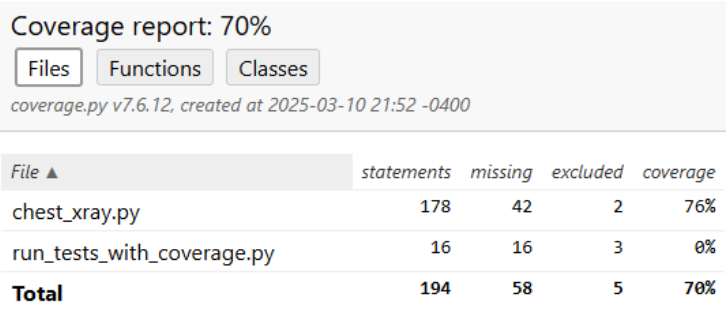
\includegraphics[width=\textwidth]{codecoverage.png}

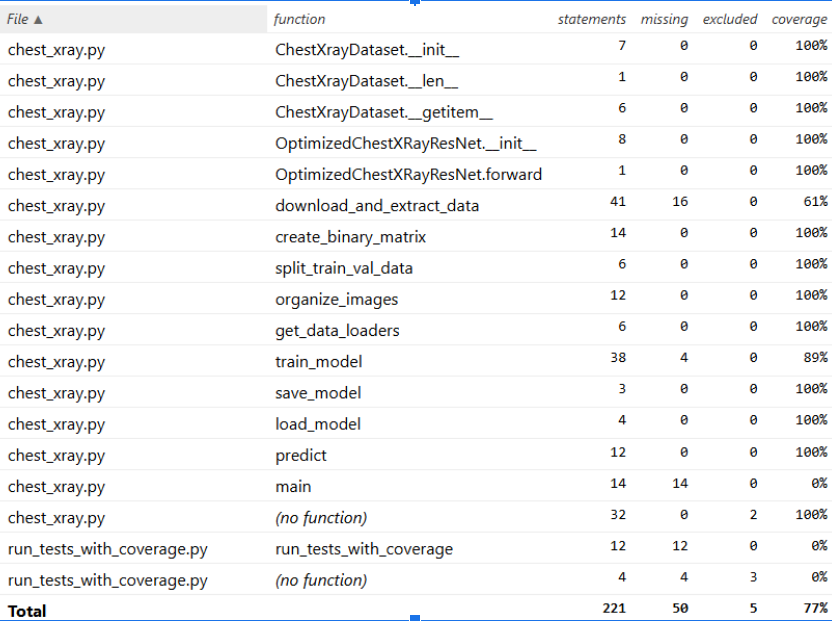
\includegraphics[width=\textwidth]{tests.png}


Overall, the system demonstrates a high degree of code coverage, ensuring that most critical paths and edge cases have been tested. Any gaps in coverage will be addressed in future iterations of testing.

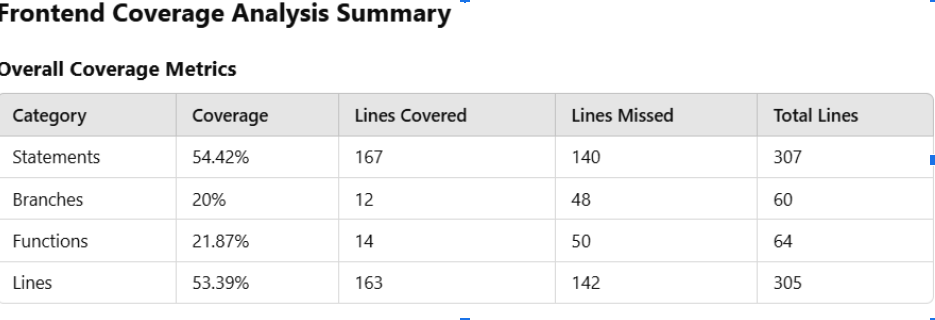
\includegraphics[width=\textwidth]{overallcoverage.png}


Frontend test coverage stands at 54.42\% for statements, 20\% for branches, 21.87\% for functions, and 53.39\% for lines, indicating gaps in authentication, API integration, and file processing. The API service has the lowest coverage at 21.9\%, missing tests for authentication handling, login, registration, image analysis, and token management (Lines 48-54, 59-152). The ModelPage component (52.63\%) lacks tests for drag-and-drop (Lines 88-89), file validation (Line 93), error handling (Lines 97-100), processing states (Lines 105-106), and API response handling (Lines 111-134, 149-176).

The Register component (58.82\%) is missing validation logic (Lines 56-72) and registration handling (Lines 90-110). The Login component (64.28\%) lacks coverage for form submission (Lines 53-66) and API error handling (Lines 86-96). ModelDetail (95.65\%) and Navbar (88.23\%) have high coverage but are missing error boundary handling (Line 100) and mobile menu interactions (Lines 60-61), respectively. Styled Components are fully covered at 100\%.

Increasing test coverage for API services, form validation, and error handling will significantly improve reliability and ensure better handling of real-world scenarios.


\bibliographystyle{plainnat}
\bibliography{../../refs/References}

\newpage{}


\section{Failed Test Cases and Debugging Actions}
% Feedback addressed - add failed test cases that occurred
During testing, a few failures were observed, especially in early iterations. The table below summarizes the failed test cases, their root causes, and the resolutions implemented to fix it in the final product:

\begin{table}[h!]
\centering
\begin{tabular}{|p{2cm}|p{3cm}|p{4cm}|p{4.5cm}|}
\hline
\textbf{Test Case} & \textbf{Description} & \textbf{Failure Cause} & \textbf{Resolution} \\
\hline
FRTC5 & No model prediction output & Sigmoid layer was applied twice, causing all predictions to be drastically scaled down and were below the threshold & Remove the extra sigmoid layer and adjusted model output scaling to have a normal probability distribution from 0-1. \\
\hline
FRTC22 & API handling of invalid image format & Initial implementation returned generic 500 error on invalid file types & Implemented MIME type validation and structured JSON error responses for unsupported formats \\
\hline
FRTC6 & Model prediction for healthy patients & Model confidently predicted disease in healthy cases & Introduced custom loss function penalizing confident false positives and removed the image labels that had too few samples (Hernia) from the dataset. Retrained model on balanced dataset. \\
\hline
\end{tabular}
\caption{Summary of Failed Test Cases and Corrective Actions}
\label{tab:failed-tests}
\end{table}



\section*{Appendix --- Reflection}

The information in this section will be used to evaluate the team members on the
graduate attribute of Reflection.

The purpose of reflection questions is to give you a chance to assess your own
learning and that of your group as a whole, and to find ways to improve in the
future. Reflection is an important part of the learning process.  Reflection is
also an essential component of a successful software development process.  

Reflections are most interesting and useful when they're honest, even if the
stories they tell are imperfect. You will be marked based on your depth of
thought and analysis, and not based on the content of the reflections
themselves. Thus, for full marks we encourage you to answer openly and honestly
and to avoid simply writing ``what you think the evaluator wants to hear.''

Please answer the following questions.  Some questions can be answered on the
team level, but where appropriate, each team member should write their own
response:


\begin{enumerate}
  \item What went well while writing this deliverable? 
  \item What pain points did you experience during this deliverable, and how
    did you resolve them?
  \item Which parts of this document stemmed from speaking to your client(s) or
  a proxy (e.g. your peers)? Which ones were not, and why?
  \item In what ways was the Verification and Validation (VnV) Plan different
  from the activities that were actually conducted for VnV?  If there were
  differences, what changes required the modification in the plan?  Why did
  these changes occur?  Would you be able to anticipate these changes in future
  projects?  If there weren't any differences, how was your team able to clearly
  predict a feasible amount of effort and the right tasks needed to build the
  evidence that demonstrates the required quality?  (It is expected that most
  teams will have had to deviate from their original VnV Plan.)


  \subsubsection{Answer}
  \section{Verification and Validation (VnV) Plan Revisions}

  \subsection{Security Compliance Verification Revisions}
  
  Originally, in our VnV Plan, under non-functional requirements, we had stated that our website needed to be compliant with data security standards, particularly those related to patient data protection, including secure storage, access controls, and adherence to privacy regulations (e.g., HIPAA). However, as we progressed, we realized that storing uploaded CXR images was unnecessary. Users, most likely radiologists or researchers, would only be looking for short-term insights, meaning long-term data storage would not only be an unnecessary cost but also irrelevant to their needs. 
  
  Instead, we decided to use SHA encryption for user account details, ensuring that in future refactoring of the website, any data shared by users would also be SHA encrypted and only stored in temporary storage, such as Redis Cache, before being deleted. This was our key revision regarding security compliance verification.

  For context, HIPAA (Health Insurance Portability and Accountability Act) is a U.S. law that governs the protection of sensitive patient health information. It ensures that personal health data is kept private and secure when stored, processed, or transmitted by healthcare providers, insurers, and associated service providers.

  Key rules include limiting access to PHI (personal health info), securing electronic data (ePHI), and notifying patients of breaches. Patients also have the right to access and correct their data.

  To implement HIPAA compliance, systems should encrypt data at rest and in transit, use access controls like role-based permissions, and maintain audit logs to track data access. Physical and network security measures must be in place, and staff should be trained in HIPAA policies. Any third-party services handling PHI must sign Business Associate Agreements (BAAs) to ensure compliance throughout the data chain.
  
  \subsection{Backend Testing and Unit Test Revisions}
  
  In the VnV plan, we made no discussion of Postman backend testing. Although we discussed unit testing at length, the actual backend testing that we conducted was primarily successful through Postman testing. For each URL belonging to the backend API, we tested each repeatedly, assuming valid and invalid payloads and credentials. This allowed us to achieve complete test coverage as well as perform tests we otherwise wouldn't have been able to conduct via the frontend or through a collective demo.
  
  Additionally, in our VnV plan, we had several unit tests, such as \texttt{FRTC3} and \texttt{FRTC4}, which ultimately had to be removed. This was due to a change in our project's goals. Initially, we aimed to build a diffusion model project to generate CXR images, but we transitioned to developing a web application for multiclass classification on CXR images. As a result, these unit tests were no longer relevant and were removed.
  
  \subsection{Challenges in Anticipating Project Direction}
  
  These particular changes were not obvious beforehand and arose due to a shift in the project's direction. Ideally, we would like to say that we could not have anticipated this, but at the time of writing the VnV document, we were already aware of potential challenges with our initial approach. As we were actively exploring solutions, it would have been beneficial to design unit tests that were more general or dynamic tests that were adaptable to changing project contexts rather than being static. 
  
  This approach would have ensured that the initial VnV plan remained useful even if the project evolved. However, there is also an argument that a verification plan that is too abstract could lose its usefulness. In hindsight, given the nature of our project, adopting a more flexible verification approach could have been a valuable revision.
  
  \subsection{What Went Well}
  
  \textbf{Gurnoor:} As a team, we distributed our roles across the document optimally. No one person was exclusive to a particular section, although each of us was primarily responsible for one section. We were all involved across different sections, helping each other and discussing any questions or confusion that arose.
  
  \textbf{Harrison:} I think we did well in reflecting on our work throughout the project. This reflection was not only limited to the appendix but also extended to addressing changes that occurred, particularly in Section 7. We encountered many obstacles throughout this project, and writing this document allowed us to address them with hindsight, which I found valuable.
  
  \textbf{Ahmed:} We did well as a team in organizing ourselves. Some of us were highly knowledgeable when it came to addressing previous unit tests and code testing, whether functional tests or coverage tests. Others were confident in handling areas such as user feedback or supervisor feedback. By playing to our strengths, we were able to put together the document in the best way possible.
  
  \textbf{Hamza:} Addressing the project changes went really well. In our earlier documents, we had outlined a different direction than the one we ultimately achieved. This wasn't necessarily a bad thing. By acknowledging these changes in Section 7, we were able to extract valuable learnings for the future. Additionally, we cleared up a lot of confusion regarding earlier misalignments in our product's function.
  
  \textbf{Jared:} I believe writing and structuring our traceability matrix went quite well. We created a framework that allowed us to quickly gauge our progress in an easily understandable manner, and we did so with high accuracy. Additionally, the automated testing section was well-executed, capturing everything we aimed to achieve in ensuring correct testing practices beyond manual testing and demos.
  
  \subsection{Challenges and Their Resolutions}
  
  One of the biggest challenges we faced was time management, especially as the project progressed and required integrating new changes. Balancing coursework alongside this deliverable sometimes made deadlines feel overwhelming. To resolve this, we divided tasks into smaller sections and held regular check-ins to ensure no team member was overloaded. This helped us stay on track without compromising the quality of critical sections.
  
  With multiple team members working on different sections, ensuring consistency in terminology, formatting, and tone became a challenge. At one point, we noticed that some sections referenced outdated features while others reflected our latest changes. To address this, we conducted a final review session where each team member reviewed a section they hadn't written. This process helped us flag inconsistencies and align all references with our final implementation.
  
  \subsection{Sources of Input for This Document}
  
  \subsubsection{Sections Stemming from Client or Peer Discussions}
  
  \textbf{Functional Requirements (Section 3):} Many of our functional requirements, such as \texttt{FR.8} (User Authentication) and \texttt{FR.1} (Image Upload), were shaped by discussions with peers and test users. Their feedback helped clarify expectations regarding user interactions and essential features. Feedback from our Rev 0 demo was particularly influential in shifting our project toward CXR classification rather than image generation.
  
  \textbf{Testing and System Refinements (Section 7 - Changes Due to Testing):} Feedback from test users and our supervisor led to significant modifications 
  
  

\end{enumerate}

\end{document}